\section{Implementierung}

\subsection{Quantenalgorithmus}
Wie im Kapitel~\ref*{Funktionsweise} zur Funktionsweise erklärt,
wird für die Periodenbestimmung die Quanten-Phase-Estimation genutzt.

Um den Quanten-Phase-Estimation Algorithmus für die Periodenberechnung zu nutzen,
benötigt man ein Gatter \(U\) welches die modulare Multiplikation \(U\ket{y} = \ket{ay \mod N}\), 
als eine unitär Transformation realisiert.
Mit den passenden \(U\)-Gatter wird der Quantenschaltkreis wie in Abbildung~\ref{fig:shor_n_qubit} strukturiert.
\begin{figure}
    \caption{QPE für Shor~\cite{anonymousket}}
    \label{fig:shor_n_qubit}
    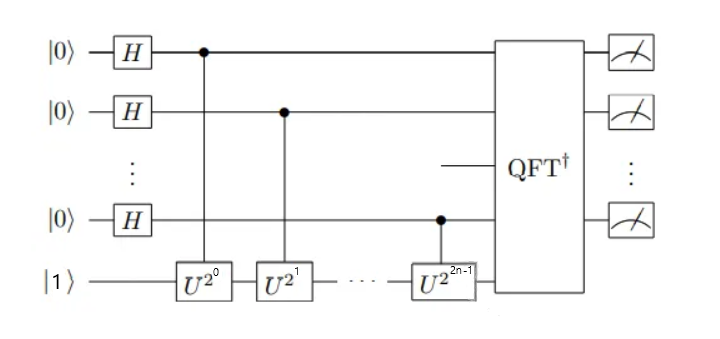
\includegraphics[width=\columnwidth]{shor_n_qubit.png}
    \centering
    \end{figure}

Die Realisierung der Transformation bedingt die Implementierung einiger arithmetischer Operationen in Form eines Quantenschaltkreises. 
Diese fungieren als Bausteine, die zusammengesetzt zur Konstruktion des übergeordneten Quantenschaltkreises für die modulare Multiplikation beitragen. 
Zu den erforderlichen arithmetischen Operationen gehört die Addition, Subtraktion sowie die modulare Addition.

In den folgenden Abschnitten werden die untergeordneten arithmetischen Operationen bis hin zur modularen Multiplikation implementiert.

\subsubsection{Addition}
Der Quantenschaltkreis für die Addition bildet das Fundament der \(U\)-Gatter und 
stellt einen der am häufigsten verwendeten Bausteine dar. 
Deswegen hat die Implementierung der Addition einen erheblichen Einfluss auf den Ressourcenbedarf des gesamten Quantenalgorithmus
und sollte daher möglichst effizient implementiert werden.

Eine Möglichkeit, die Addition als Quantenschaltkreis zu realisieren, 
besteht im Nachbau eines klassischen Schaltkreises aus Volladdierern. 
Da es nicht möglich ist, 
die notwendige klassischen Gatter wie AND und OR als unitäre Transformation mit nur zwei Qubits darzustellen~\cite{Hoever2023QC},
werden zusätzliche Hilfsqubits benötigt.
Die zusätzlichen Hilfsqubits bewirken, dass der Nachbau eines klassischen Schaltkreis für die Addition zweier \(n\)-Bit Zahlen, 
also solche der Größenordnung \(2^n\), mindestens \(3n\) Qubits benötigt~\cite{zalka1998fast}.

Eine effizientere Methode, die ohne Hilfsqubits auskommt, ist die Quanten-Addition~\cite{draper2000addition}. 
Die Quanten-Addition führt die Berechnung auf quantenmechanische Weise durch. 
Im Wesentlichen wird dabei die Addition in der Fourier-Basis berechnet, 
wobei die Phasen der Qubits eines Summanden mit kontrollierte Phasenverschiebungen auf die Qubits des anderen Summanden wirkt.

Im Folgenden wird ein Beispiel für die Quanten-Addition zweier Qubit-Register \(\ket{a}_3\) und \(\ket{b}_3\), 
jeweils bestehend aus drei Qubits, betrachtet:
\begin{figure}[H]
    \caption{Quantum-Addition}
    \label{fig:3_qubit_quantum_add}
    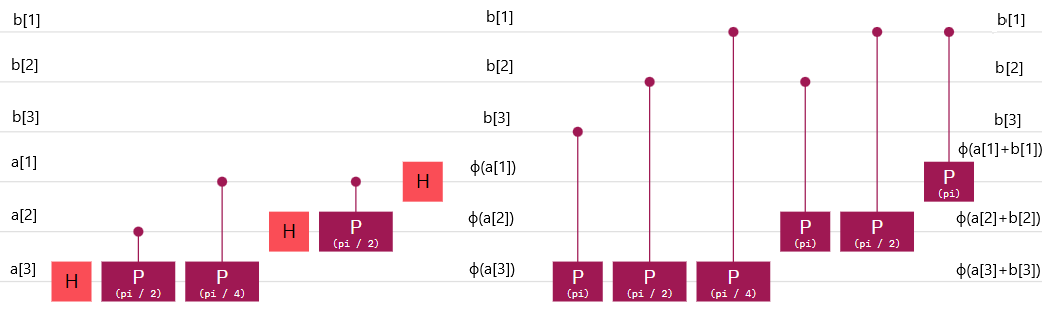
\includegraphics[width=\columnwidth]{3_qubit_quantum_add.png}
    \centering
    \end{figure}
Die Registermarkierungen in der Mitte von Abbildung~\ref*{fig:3_qubit_quantum_add} unterteilen die Darstellung in zwei Hälften.
Die linke Hälfte repräsentiert die Quanten-Fourier-Transformation, 
während die rechte Hälfte die Quanten-Addition zeigt.

Wie man an der Struktur der Quanten-Addition erkennen kann,
ist die Anordnung der Gatter fast identisch mit der Quanten-Fourier-Transformation.
Ein Unterschied besteht darin, 
dass die Hadamard-Gatter durch kontrollierte \(P(\pi)\) Phasen-Gatter ersetzt wurden.
Sowohl das Hadamard-Gatter als auch das \(P(\pi)\) Phasen-Gatter erzeugen eine relative Phase von \(e^{\pi i}\).
Ein weiterer Unterschied zur Quanten-Fourier-Transformation besteht darin, 
dass die Phasen-Gatter nicht durch das gleiche Register\(\ket{a}_3\) kontrolliert werden, 
auf das die Gatter auch wirken.
Stattdessen kontrollieren die Qubits des Registers \(\ket{b}_3\) die Phasen-Gatter.
Dabei wird das \(P(\pi)\) Phasen-Gatter durch das Qubit des \(\ket{b}_3\) kontrolliert,
welches die selbe Wertigkeit hat wie das Zielqubit des \(\ket{a}_3\) Registers.
Jedes weitere kontrollierte Phasen-Gatter für das gleiche Zielqubit 
wird fortlaufend von dem nächstkleineren Qubit von \(\ket{b}_3\) kontrolliert.

Im Prinzip handelt es sich bei dieser Quantenschaltung um eine Anwendung derselben Phasenverschiebungen 
wie bei der Quanten-Fourier-Transformation. 
Der grundlegende Unterschied liegt darin, 
dass diese Phasenverschiebungen kontrolliert auf ein anderes Quantenregister angewendet werden.

Die Wirkung der Quanten-Addition wird anhand der Abbildung~\ref*{fig:3_qubit_quantum_add} verdeutlicht:
Am Anfang der linken Hälfte befinden sich beide Register in der Standardbasis.
Auf das Zielregister \(\ket{a}_3\) wirkt die Quanten-Fourier-Transformation ohne Swap Gatter.
Dadurch befindet sich \(\ket{a}_3\) nun in der Fourier-Basis \(\Phi\), also \(\ket{\Phi(a)}_3\):
\[\ket{\Phi(a)}_3 = \frac{1}{\sqrt{8}} [ (\ket{0} + { e^{\frac{2 \pi i (2^0a_1)}{2^1}}}\ket{1} ) \Tensor
( \ket{0} + { e^{\frac{2 \pi i (2^1a_2+2^0a_1)}{2^2}}}\ket{1} ) \Tensor
( \ket{0} + { e^{\frac{2 \pi i (2^{2}a_3 +2^1a_2+2^0a_1)}{2^3}}}\ket{1} ) ] \]
Anschließend wirkt auf das hinterste Tensorprodukt ein \(P(\pi)\) Phasen-Gatter,
welches durch \(\ket{b_3}_1\) kontrolliert wird.
Wenn sich \(\ket{b_3}_1\) im Zustand \(\ket{0}_1\) befindet, passiert nichts.
Wenn es sich im Zustand \(\ket{1}_1\) befindet, dass das Phasen-Gatter angewendet wird.
Dieses Verhalten kann man für beide Fälle mit den entsprechenden Matrizen 
\(\begin{pmatrix}
    1 & 0 \\
    0 & e^{\pi i b_3}
  \end{pmatrix}\)
  beziehungsweise  
  \(\begin{pmatrix}
    1 & 0 \\
    0 & e^{\frac{2\pi i (2^2b_3)}{2^3}}
  \end{pmatrix}\)
beschreiben.
Schreibt man das hinterste Tensorprodukt als Vektor, ergibt sich die folgende Formulierung:
\[\frac{1}{\sqrt{2}}( \ket{0} + { e^{\frac{2 \pi i (2^{2}a_3 +2^1a_2+2^0a_1)}{2^3}}}\ket{1}) \equiv
\frac{1}{\sqrt{2}}
\begin{pmatrix}
     1  \\
     e^{\frac{2 \pi i (2^{2}a_3 +2^1a_2+2^0a_1)}{2^3}}
  \end{pmatrix}
    \]
Dann wird durch das Ergebnis der Verrechnung mit dem Phasen-Gatter deutlich, 
dass die Addition im Wesentlichen in der Phase des Quantenzustands stattfindet:
\[\begin{pmatrix}
    1 & 0 \\
    0 & e^{\frac{2\pi i (2^2b_3)}{2^3}}
  \end{pmatrix}
    \cdot
\frac{1}{\sqrt{2}}
\begin{pmatrix}
    1  \\
     e^{\frac{2 \pi i (2^{2}a_3 +2^1a_2+2^0a_1)}{2^3}}
  \end{pmatrix}
  =
  \frac{1}{\sqrt{2}}
  \begin{pmatrix}
    1  \\
     e^{\frac{2 \pi i (2^{2}(a_3+b_3) +2^1a_2+2^0a_1)}{2^3}}
  \end{pmatrix}
\]
Wie in der Abbildung~\ref*{fig:3_qubit_quantum_add} erkenntlich,
wirken auf das hinterste Tensorprodukt auch noch die beiden Phasen-Gatter \(P(\frac{\pi}{2})\) und \(P(\frac{\pi}{4})\) mit:
\[
    P(\frac{\pi}{2}) = 
\begin{pmatrix}
    1 & 0 \\
    0 & e^{\frac{\pi}{2} i b_2}
  \end{pmatrix}
  =
  \begin{pmatrix}
    1 & 0 \\
    0 & e^{\frac{2\pi i (2^1b_2)}{2^3}}
  \end{pmatrix}
  ~;~
P(\frac{\pi}{4}) = 
\begin{pmatrix}
    1 & 0 \\
    0 & e^{\frac{\pi}{4} i b_1}
  \end{pmatrix}
  =
  \begin{pmatrix}
    1 & 0 \\
    0 & e^{\frac{2\pi i (2^0b_1)}{2^3}}
  \end{pmatrix}
\]
\[
    \begin{pmatrix}
        1 & 0 \\
        0 & e^{\frac{2\pi i (2^0b_1)}{2^3}}
      \end{pmatrix}
      \cdot
      \begin{pmatrix}
        1 & 0 \\
        0 & e^{\frac{2\pi i (2^1b_2)}{2^3}}
      \end{pmatrix}
      \cdot
      \frac{1}{\sqrt{2}}
      \begin{pmatrix}
        1  \\
         e^{\frac{2 \pi i (2^{2}(a_3+b_3) +2^1a_2+2^0a_1)}{2^3}}
      \end{pmatrix}
      =
      \frac{1}{\sqrt{2}}
      \begin{pmatrix}
        1  \\
         e^{\frac{2 \pi i (2^{2}(a_3+b_3) +2^1(a_2+b_2)+2^0(a_1+b_1))}{2^3}}
      \end{pmatrix}
\]
Wendet man alle weiteren Phasen-Gatter auf das vollstände Tensorprodukt an, 
erhält man:
\[
    \frac{1}{\sqrt{8}} [ (\ket{0} + { e^{\frac{2 \pi i (2^0(a_1+b_1))}{2^1}}}\ket{1} ) \Tensor
( \ket{0} + { e^{\frac{2 \pi i (2^1(a_2+b_2)+2^0(a_1+b_1))}{2^2}}}\ket{1} ) \Tensor
( \ket{0} + { e^{\frac{2 \pi i (2^{2}(a_3+b_3) +2^1(a_2+b_2)+2^0(a_1+b_1))}{2^3}}}\ket{1} ) ]
\]
Setzt man in diese Formel zwei Zahlen in Binärschreibweise ein, 
wird man den selben Zustand erhalten,
wie wenn man die Summe der beiden Zahlen in die Formel der Quanten-Fourier-Transformation einsetzt.
Beispielsweise sei \(a = 3\) also binär \(a_3 = 0\), \(a_2 = 1\),\(a_1 = 1\) und 
\(b = 1\) also \(b_3 = 0\), \(b_2 = 0\),\(b_1 = 1\):
\[
\frac{1}{\sqrt{8}} [ (\ket{0} + { e^{\frac{2 \pi i (2^0(1+1))}{2^1}}}\ket{1} ) \Tensor
( \ket{0} + { e^{\frac{2 \pi i (2^1(1+0)+2^0(1+1))}{2^2}}}\ket{1} ) \Tensor
( \ket{0} + { e^{\frac{2 \pi i (2^{2}(0+0) +2^1(1+0)+2^0(1+1))}{2^3}}}\ket{1} ) ]
\]
\[
=\frac{1}{\sqrt{8}} [ (\ket{0} + \ket{1} ) \Tensor
( \ket{0} +   \ket{1} ) \Tensor
( \ket{0} +  e^{\pi i }\ket{1} ) ]
\]
Das dies tatsächlich die Summe in Fourier-Basis entspricht, 
wird deutlich wenn man das selbe Tensorprodukt aus der Quanten-Fourier-Transformation bildet:
\[
    QFT(\ket{c}_3)
    \frac{1}{\sqrt{8}} [ (\ket{0} + { e^{\frac{2 \pi i (2^0(c_1))}{2^1}}}\ket{1} ) \Tensor
( \ket{0} + { e^{\frac{2 \pi i (2^1(c_2)+2^0(c_1))}{2^2}}}\ket{1} ) \Tensor
( \ket{0} + { e^{\frac{2 \pi i (2^{2}(c_3) +2^1(c_2)+2^0(c_1))}{2^3}}}\ket{1} ) ]
\]
Die Summe von \(a\) und \(b\) entspricht \(c = 4\) also \(c_3 = 1,~c_2 = 0,~c_1=0\):
\[
    QFT(\ket{4}_3)
    \frac{1}{\sqrt{8}} [ (\ket{0} + { e^{\frac{2 \pi i (2^0(0))}{2^1}}}\ket{1} ) \Tensor
( \ket{0} + { e^{\frac{2 \pi i (2^1(0)+2^0(0))}{2^2}}}\ket{1} ) \Tensor
( \ket{0} + { e^{\frac{2 \pi i (2^{2}(1) +2^1(0)+2^0(0))}{2^3}}}\ket{1} ) ]
\]
\[
    = 
    \frac{1}{\sqrt{8}} [ (\ket{0} + { e^{\frac{2 \pi i (0)}{2^1}}}\ket{1} ) \Tensor
( \ket{0} + { e^{\frac{2 \pi i (0)}{2^2}}}\ket{1} ) \Tensor
( \ket{0} + { e^{\frac{2 \pi i (2^{2}(1))}{2^3}}}\ket{1} ) ]
\]
\[
=\frac{1}{\sqrt{8}} [ (\ket{0} + \ket{1} ) \Tensor
( \ket{0} +   \ket{1} ) \Tensor
( \ket{0} +  e^{\pi i }\ket{1} ) ]
\]
Das Ergebnis der Quanten-Addition zweier Summanden \(a=3,~b=1\), 
jeweils in einem Register mit drei Qubits,
ist somit identisch mit dem Zustand, 
der durch die Anwendung der Quanten-Fourier-Transformation auf ein Register 
aus ebenfalls drei Qubits mit der Summe der beiden Zahlen entsteht.

Mit einer anschließenden inversen Quanten-Fourier-Transformation, 
kann die Summe in die Standardbasis und somit in einen Messbaren Zustand transformiert werden:
\[
iQFT(\ket{\Phi(4)_3})
\equiv
 iQFT(\frac{1}{\sqrt{8}} [ (\ket{0} + \ket{1} ) \Tensor
( \ket{0} +   \ket{1} ) \Tensor
( \ket{0} +  e^{\pi i }\ket{1} ) ]) 
=
\ket{4}_3
\]

Das Zielregister sollte aus genügend Qubits bestehen, 
damit die Summe vollständig erfasst werden kann.
Andernfalls kommt es zum overflow mit \(a + b \mod 2^n\), 
wobei \(n\) die Anzahl an Qubits des Zielregisters beschreibt~\cite{beauregard2003circuit}.

Für die Realisierung der modularen Multiplikation wird zu keinem Zeitpunkt der Berechnung eine Addition zweier Zwischenergebnisse benötigt. 
Genauer gesagt, ist es nicht nötig, ein Quantenregister auf ein anderes zu addieren. 
Stattdessen wird die Quanten-Addition benutzt, um eine vorab bekannte Zahl auf ein Quantenregister zu addieren.

Bei der Quanten-Addition mit zwei Register wie in Abbildung~\ref{fig:3_qubit_quantum_add} erfolgt die Phasenverschiebung kontrolliert,  
also in Abhängigkeit des Inhaltes von Register \(\ket{b}_3\).
Ist der Inhalt von Register \(\ket{b}_3\) vorab bekannt,
können gewöhnliche Phasen-Gatter anstelle von kontrollierten verwendet werden~\cite{beauregard2003circuit}.

Wenn bei der Quanten-Addition mit zwei Registern ein Phasen-Gatter aufgrund des zugehörigen Kontrollqubits im Zustand \(\ket{1}\) angewendet wird,
wird es in der Variante mit einem einzelnen Register als gewöhnliches Phasen-Gatter verwendet.
Ist das Kontrollqubit hingegen im Zustand \(\ket{0}\), 
wodurch das Phasen-Gatter bei der Quanten-Addition mit zwei Registern nicht zur Anwendung kommt, 
wird dieses Phasen-Gatter in der Variante mit nur einem Register weggelassen.

\begin{figure}[H]
    \caption{Quantum-Addition fixierte Phasenverschiebungen}
    \label{fig:3_qubit_fixed_quantum_addition}
    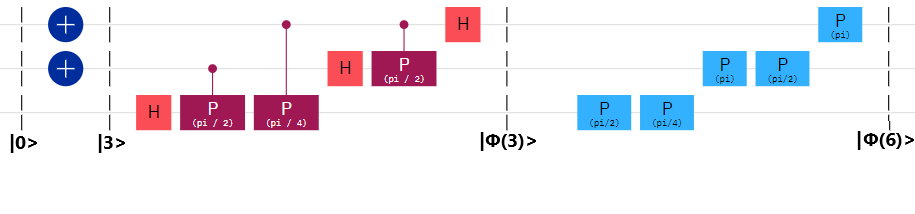
\includegraphics[width=\columnwidth]{3_qubit_fixed_quantum_addition.png}
    \centering
    \end{figure}
In Abbildung~\ref{fig:3_qubit_fixed_quantum_addition} ist die Quanten-Addition für ein 3-Qubit Register abgebildet.
Die blauen Phasen-Gatter sorgen für die Quanten-Addition mit einem fixierten Wert von \(3\).
Vergleicht man die Abbildung~\ref{fig:3_qubit_fixed_quantum_addition} mit der Abbildung~\ref{fig:3_qubit_quantum_add} fällt auf, 
dass das aller erste Phasen-Gatter der Quanten-Addition nicht vorkommt.
Im Quantenschaltkreis der Abbildung~\ref{fig:3_qubit_quantum_add} würde ein Registerinhalt von \(b = 3\) das Kontrollqubit \(b_3\) nicht setzen. 
Somit kommt das erste Phasen-Gatter der Quanten-Addition nicht zum Einsatz und 
wird deswegen in der Variante wie in Abbildung~\ref{fig:3_qubit_fixed_quantum_addition} weggelassen. 

Des weiteren ist es möglich, 
den Quantenschaltkreis der Quanten-Addition für eine vorab festgelegte Zahl ressourcensparender zu realisieren.
Die Optimierung bezieht sich dabei auf die Anzahl der verwendeten Gatter.
Wird die Quanten-Addition für eine feste Zahl realisiert, 
können für jedes einzelne Qubit die angewendeten Phasenverschiebungen vorab zusammengerechnet werden.
Demnach bietet es sich an, 
die zusammengerechneten Phasenverschiebung in ein einzelnes Phasen-Gatter zusammen zu fassen.
Nach diesem Prinzip, benötigt man für eine Quanten-Addition maximal ein einzelnes Phasen-Gatter pro Qubit.

\begin{figure}[H]
  \caption{Ressourcensparende Quantum-Addition}
  \label{fig:3_qubit_fixed_quantum_addition_opt}
  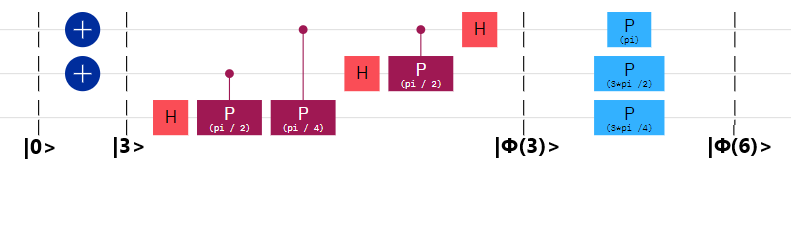
\includegraphics[width=\columnwidth]{3_qubit_fixed_quantum_addition_opt.png}
  \centering
  \end{figure}
Der Quantenschaltkreis in Abbildung~\ref{fig:3_qubit_fixed_quantum_addition_opt} führt die identische 
Berechnung durch, wie der Quantenschaltkreis aus Abbildung~\ref{fig:3_qubit_fixed_quantum_addition}.
Darüber hinaus, werden die benötigten Phasenverschiebungen mit einem einzigen Phasen-Gatter pro Qubit realisiert.

Die Implementierung nutzt die ressourceneffiziente Variante der Quanten-Addition.
In der Funktion \texttt{A\_Gate} wird ein Gatter erzeugt, 
das sämtliche für die Quanten-Addition erforderlichen Phasen-Gatter umfasst.
Der Code zur Funktion ist in Abbildung~\ref{code:QuantumAdd} dargestellt.
\begin{figure}[H]
  \caption{Quantum-Addition in Qiskit}
  \label{code:QuantumAdd}
\begin{minted}[linenos,fontsize=\footnotesize]{python}    
def A_Gate(a_bin: list[int]) -> qiskit.circuit.gate:
    A_Gate = qiskit.QuantumCircuit(len(a_bin))
    theta_list = [0.0]*len(a_bin)
    for target_bit in range(len(a_bin)):
        exponent = 1
        for control_bit in reversed(range(target_bit+1)):
            if a_bin[control_bit] == 1:
                theta_list[target_bit]+= 2*pi/(2**(exponent))
            exponent+=1
    for qubit_index in range(len(a_bin)):
        A_Gate.append(P_Gate(theta_list[qubit_index]),[qubit_index])
    A_Gate = A_Gate.to_gate()
    A_Gate.name = " Add(" + str (binToDez(a_bin) )+ ")"
    return A_Gate 
  \end{minted}
\end{figure}
Der Funktion \texttt{A\_Gate} wird der zu addierende Summand im Binärformat übergeben, 
wobei am Index Null das Least-Significant-Bit liegt.
Abhängig von der Anzahl der Bits des Summanden wird ein Quantenschaltkreis mit der gleichen Anzahl an Qubits erzeugt. 
In den Zeilen 4 bis 9 werden die Phasenverschiebungen, die auf ein einzelnes Qubit wirken sollen, berechnet und akkumuliert.
Anschließend wird in den Zeilen 10 bis 11 auf jedes Qubit des Quantenschaltkreises ein individuelles Phasen-Gatter angewendet.
Die Phasenverschiebung eines einzelnen Phasen-Gatters ergibt sich aus der vorherigen Akkumulation in den Zeilen 4 bis 9.
Abschließend wird der Quantenschaltkreis in ein Gatter umgewandelt und mit einer passenden Bezeichnung versehen.

\subsubsection{Subtraktion}
Die Quanten-Addition besteht ausschließlich aus unitären Gattern 
und ist daher selbst auch unitär. 
Diese Eigenschaft vereinfacht die Implementierung der Subtraktion. 
Indem die Quanten-Addition invertiert wird, ergibt sich ein Quantenschaltkreis, 
der eine Subtraktion in der Fourier-Basis ausführt. 
Damit hat man praktisch einen Quantenschaltkreis der Quanten-Subtraktion.

Genau wie bei der Quanten-Addition kann es auch bei der Quanten-Subtraktion zu einem Overflow,
beziehungsweise im konkreten Kontext, zu einem Underflow kommen.
Bei der Quanten-Subtraktion tritt dieser Effekt ein, 
falls der Minuend im Zielregister kleiner als der Subtrahend ist.

Dieser Effekt kann verwendet werden, um herauszufinden, 
ob der Subtrahend größer ist als der Minuend~\cite{beauregard2003circuit}.
Angenommen man hat zwei Zahlen die maximal der Größenordnung \(2^n\) entsprechen und 
ein Zielregister welches aus \(n+1\) Qubits besteht.
Der Subtrahend \(b\) befindet sich im Zielregister also \(\ket{\phi(b)}_{n+1}\), 
worauf die Quanten-Subtraktion mit dem Minuend \(a\) wirkt.
Dann existieren zwei mögliche Fälle:
\[b \geq a~\rightarrow~\ket{\phi(b-a)}_{n+1};~
b < a~\rightarrow~\ket{\phi(2^{n+1}-(a-b))}_{n+1}
  \]
Das Most-Significant Bit ist ausschließlich im zweiten Fall gesetzt und kann somit, 
nachdem das Register in die Standardbasis transformiert wird, 
als eine Art Borrow-Bit entspricht.

Die Implementierung der Quanten-Subtraktion ist aufgrund der \texttt{inverse} Funktion von Qiskit unkompliziert.
Wendet man die \texttt{inverse} Funktion auf ein Gatter der Quanten-Addition der \texttt{A\_Gate} Funktion an, 
wird dieses in die Quanten-Subtraktion invertiert.
Der Code davon ist in~\ref{code:QuantumSub} abgebildet.
\begin{figure}[H]
  \caption{Quantum-Subtraktion in Qiskit}
  \label{code:QuantumSub}
\begin{minted}[linenos,fontsize=\footnotesize]{python}    
def S_Gate(subtrahend_bin: list[int]) -> qiskit.circuit.gate:
    S_Gate = A_Gate(subtrahend_bin).inverse()
    S_Gate.name = "  Sub(" + str (binToDez(subtrahend_bin) )+ ")"
    return S_Gate
  \end{minted}
\end{figure}

\subsubsection{Modulare Addition} \label{sub:modulareAddition}
Die Gatter der Quanten-Addition und der Quanten-Subtraktion ermöglichen die Konstruktion einer unitären Transformation, 
die die Berechnung der modularen Addition realisiert.
Gemeinsam bilden sie einen Quantenschaltkreis, 
der das Ergebnis der Berechnung \(\ket{\Phi(a+b)\mod N}\) für \(a, b < N\) im Zielregister speichert.

\begin{figure}[H]
  \caption{Modulare Addition nach Beauregard~\cite{beauregard2003circuit}}
  \label{fig:modulare_addition_paper}
  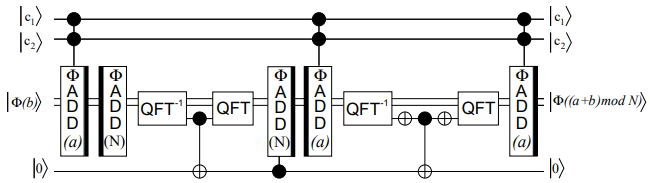
\includegraphics[width=\columnwidth]{Modular_adder_Paper.PNG}
  \centering
  \end{figure}
Abbildung~\ref{fig:modulare_addition_paper} zeigt das verwendete Konzept, 
das für die Implementierung der modularen Addition als Bauplan diente.
In der Grafik sind zwei Arten von \(\phi ADD\)-Gattern zu sehen.
Dabei handelt es sich um die Quanten-Addition, erkennbar mit dem fettgedruckten Strich auf der rechten Seite und 
der Quanten-Subtraktion mit einem fettgedruckten Strich auf der linken Seite.
Sowohl die Quanten-Addition als auch die Quanten-Subtraktion addieren beziehungsweise subtrahieren eine fixe Zahl und 
sind somit die zuvor vorgestellten Varianten mit gewöhnlichen Phasen-Gattern.
Der Quantenschaltkreis zur modularen Addition agiert als Baustein in einem größeren Gesamtbild, 
weshalb die zwei Kontroll-Qubits \(\ket{c_1}\) und \(\ket{c_2}\) eingebaut werden, 
die im weiteren Verlauf Anwendung finden.
Das Eingaberegister stellt auch das Zielregister dar und 
ist initial bereits in der Fourier-Basis mit \(\ket{\phi(b)}\).
Das Zielregister wird um ein weiteres Qubit erweitert, 
welches das Most-Significant-Bit des Zielregisters dargestellt.
Dieses Qubit hat einen besonderen Anwendungszweck und wird im weiteren als Borrow-Qubit bezeichnet.
Insgesamt besteht das Zielregister also aus \(n+1\) Qubits wenn der Modulus \(N\) einer Größenordnung von \(2^n\) entspricht.
Alle nachhaltigen Veränderungen durch den Quantenschaltkreis betreffen ausschließlich das Zielregister.
Des Weiteren verwendet die Quantenschaltung noch ein Qubit, welches initial im Zustand \(\ket{0}\) beginnt.
Der Zustand dieses einzelnen Qubits bedingt eine Fallunterscheidung in der Berechnung des Quantenschaltkreises und 
wird daher im Weiteren als Bedingungs-Qubit bezeichnet. 

Um die Berechnung des Quantenschaltkreises nachvollziehen zu können, 
wird die Auswirkung der verwendeten Gatter im einzelnen erklärt.
Die erste Quanten-Addition sorgt dafür, 
dass auf den initialen Zielregister \(\ket{\phi(b)}\) eine Addition mit \(a\) erfolgt und 
dadurch \(\ket{\phi(b + a)}\) entspricht.
Darauf folgt eine Quanten-Subtraktion die mit dem Subtrahend \(N\) auf das Zielregister mit
\(\ket{\phi(b + a - N)}\) wirkt. 
Daraus resultieren zwei mögliche Zustände:
\[1.~(b+a) \geq N~\rightarrow~\ket{\phi((b+a) - N)}_{n+1};~2.~
(b+a) < N~\rightarrow~\ket{\phi(2^{n+1}-(N-(a+b)))}_{n+1}
  \]
Im erste Fall entspricht das Ergebnis der korrekten Berechnung von \(a+b \mod N\).
In diesem Fall ist der Registerinhalt mit \(a+b \mod N\) kleiner als \(N\), 
weshalb das Borrow-Bit nicht gesetzt ist.
Im Gegensatz dazu ist das Ergebnis im zweiten Fall fehlerhaft.
Da bei \((b+a) < N\) bereits der Rest der modularen Restklasse im Register steht, 
wird durch die Quanten-Subtraktion ein \(N\) zu viel vom Registerinhalt abgezogen.
Dadurch entsteht ein underflow im Zielregister wodurch das Borrow-Bit gesetzt wird.

Als nächstes wirkt die inverse Quanten-Fourier-Transformation auf das Zielregister und führt eine Transformation in die Standartbasis durch.
Aufgrund des Basiswechsels in die Standartbasis beschreiben die Zustände der Qubits des Zielregisters nun das Ergebnis in der Binärdarstellung.
In der Binärdarstellung befindet sich im ersten Fall das Borrow-Bit im Zustand \(\ket{0}\) und im zweiten Fall im Zustand \(\ket{1}\).
Anhand dieser Unterscheidung kann man eine bedingte Operation mittels eines kontrollierten X-Gatter realisieren.
Dafür kontrolliert das Borrow-Bit ein X-Gatter welches auf das Bedingungs-Qubit wirkt.
Dadurch wird das Bedingungs-Qubit ausschließlich im zweiten Fall in den Zustand \(\ket{1}\) versetzt.
Danach wird das Zielregister wieder in die Fourier-Basis transformiert, 
indem die Quanten-Fourier-Transformation angewendet wird.
Anschließend kontrolliert das Bedingungs-Qubit eine Quanten-Addition mit dem Summanden \(N\) auf das Zielregister.
Die kontrollierte Quanten-Addition wird also nur im zweiten Fall angewendet und korrigiert das vorher ungültige Ergebnis,
zu dem korrekte:
\[
\ket{\phi(2^{n+1}-(N-(a+b)))}_{n+1} \underrightarrow{~+N~} 
\ket{\phi(2^{n+1}+(a+b))}_{n+1} \underrightarrow{\text{overflow }2^{n+1}}
\ket{\phi(a+b)}_{n+1}
  \]
Nun befinden sich in beiden Fällen das korrekt berechnete Ergebnis im Zielregister mit \(\ket{\Phi(a+b)\mod N}\).
Somit ist die Berechnung der modularen Addition abgeschlossen.

Je nach dem, welcher der beiden Fälle eingetreten ist, befindet sich das Bedingungs-Qubit in einem anderen Zustand.
Um zu verhindern, dass sich das Bedingungs-Qubit in einem ungewissen Zustand befindet und dadurch zum "`Trash"'-Qubit wird, 
wird der initiale Zustand \(\ket{0}\) des Bedingungs-Qubit durch die restlichen Gatter des Quantenschaltkreises wiederhergestellt.
Ein eindeutiger Zustand ermöglicht, dass das Bedingungs-Qubit bei weiteren Berechnungen wiederverwendet werden kann.

Um das Bedingungs-Qubit zurückzusetzen, 
wird zuerst eine Quanten-Subtraktion mit \(a\) auf das Zielregister angewendet.
Um die Auswirkungen dieser Quanten-Subtraktion hervorzuheben, wird der Registerinhalt für beide Fälle untersucht:
Im ersten Fall war \((b+a) \geq N\) weswegen die Subtraktion von \(N\) zum Ergebnis der modularen Addition führte.
Da \(a, b < N\) gilt, ist das Ergebnis der modularen Addition kleiner als \(a\).
Die Quanten-Subtraktion mit \(a\) führt also zu einem Underflow, wodurch das Borrow-Bit gesetzt wird.
Im zweiten Fall, war \((b+a) < N\).
Deswegen wurde die Subtraktion von \(N\) nicht durchgeführt, 
beziehungsweise wieder rückgängig gemacht, da \((b+a)\) bereits das Ergebnis der modularen Addition ist.
Für den zweiten Fall gilt als Ergebnis also \((b+a)\) und dies ist größer als \(a\), 
darum kommt es zu keinem Underflow und das Borrow-Bit ist deswegen nicht gesetzt.
Der Zustand des Borrow-Bits ist nun also im Vergleich zu den Fällen des vorherigen Abschnitts der Quantenschaltung invertiert.

Um das Borrow-Bit auslesen zu können, 
wird analog zum vorherigen Abschnitt des Quantenschaltkreises eine inverse Quanten-Fourier-Transformation durchgeführt.
Anschließend wird ein X-Gatter auf das Borrow-Bit angewendet.
Dadurch befindet sich das Borrow-Bit nun in denselben Zuständen wie in den beiden Fällen des ersten Abschnitts der Quantenschaltung.
Im nächsten Schritt kontrolliert das Borrow-Bit ein X-Gatter, das auf das Bedingungs-Qubit wirkt.
Dadurch wird es wieder in den initialen Zustand \(\ket{0}\) versetzt.

Um den Zustand \(\ket{\Phi(a+b)\mod N}\) des Zielregister wiederherzustellen, 
werden die Gatter bis zur Quanten-Subtraktion mit \(a\) inverse angewendet.
Zunächst wird ein selbstinverses X-Gatter auf das Borrow-Bit angewendet.
Danach folgt die Quanten-Fourier-Transformation, 
die die Inverse der inversen Quanten-Fourier-Transformation darstellt.
Abschließend folgt die Quanten-Addition mit \(a\), 
um die zuvor erfolgte Quanten-Subtraktion von \(a\) auf das Zielregister zu revertieren.

Das Zielregisters beinhaltet nun also den gewünschten Zustand \(\ket{\Phi(a+b)\mod N}\) für \(a, b < N\).
Des weiteren befindet sich das Bedingungs-Qubit wieder im initialen Zustand und kann für weitere Rechnungen wiederverwendet werden.

\vspace{1em}

Wenn man den Quantenschaltkreis in Abbildung~\ref{fig:modulare_addition_paper} betrachtet,
fällt auf, 
dass nicht alle Quanten-Additionen und Quanten-Subtraktionen kontrolliert durchgeführt werden.
Die modulare Addition soll nur dann ausgeführt werden, wenn die Kontroll-Qubits \(\ket{c_1}\) und \(\ket{c_2}\) gesetzt sind.
Dies ist zurückzuführen auf die Bedingung \(b < N\), 
die dafür sorgt, dass der Rest des Quantenschaltkreises lediglich die Identitätstransformation durchführt, 
wenn die Kontroll-Qubits nicht aktiviert sind~\cite{beauregard2003circuit}.
Der Grund, weshalb nicht alle Quanten-Additionen, 
Quanten-Subtraktion und gegebenenfalls sogar die (inversen) Quanten-Fourier-Transformationen kontrolliert sind,
liegt in der erhöhten Komplexität, die dadurch im Quantenschaltkreis entstehen würde~\cite{beauregard2003circuit}.
Wenn ein Kontroll-Qubit nicht aktiviert ist, wird das kontrollierte Gatter zwar ausgeführt, jedoch ohne praktische Wirkung.
Abbildung~\ref{fig:gatedef_U1U2U3_CNOT} zeigt die physikalische Implementierung dreier Single-Qubit-Gatter im Vergleich zu einem kontrollierten X-Gatter.
Wie aus der Abbildung erkennbar, 
benötigt das kontrollierte Gatter mehr Hardware-Elemente als die drei Single-Qubit-Gatter.
Somit ist es nicht möglich die Komplexität des Quantenschaltkreis zu verringern, 
indem zusätzliche Gatter kontrolliert angewendet werden.

\begin{figure} [H]
  \caption{Physikalische Implementierung~\cite{ibmqx5}}
  \label{fig:gatedef_U1U2U3_CNOT}
  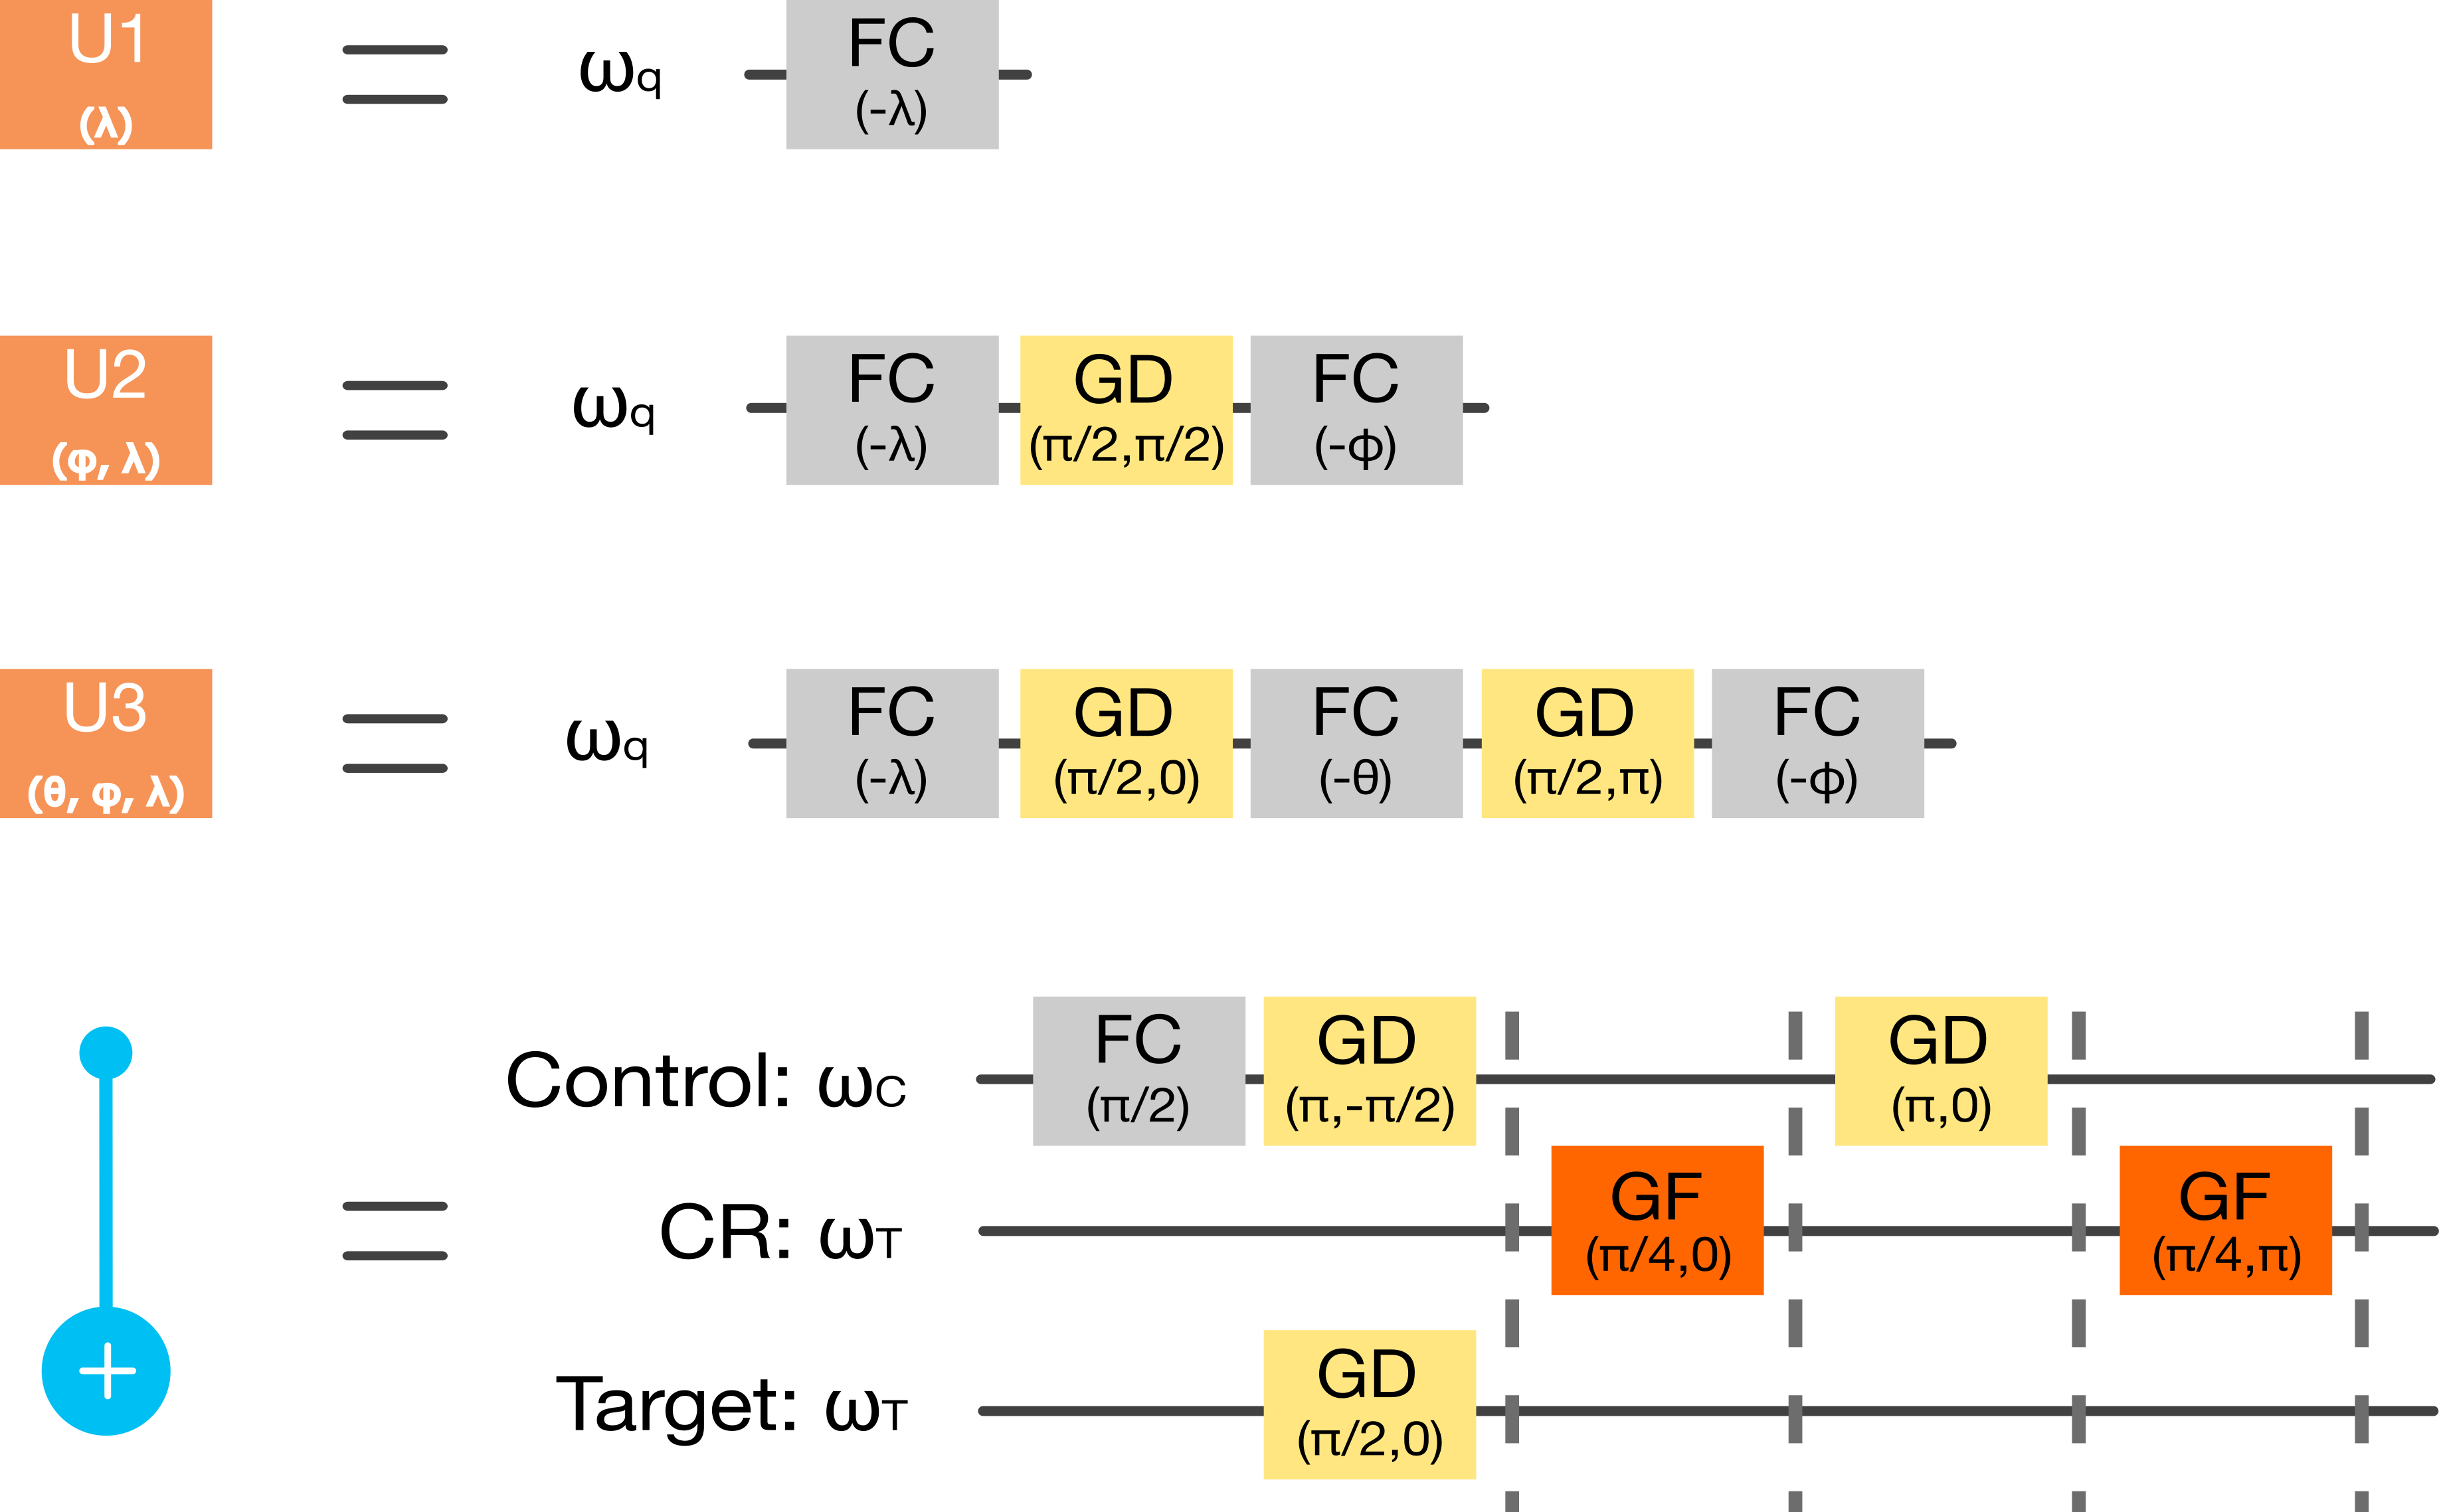
\includegraphics[scale=0.5]{gatedef_U1U2U3_CNOT.png}
  \centering
  \end{figure}

Ein weiterer Aspekt, 
der die Komplexität der Quantenschaltung für die modulare Addition erhöht, 
ist der Abschnitt, der das Bedingungs-Qubit zurücksetzt.
Wäre es möglich, diesen Teil auszulassen, könnten zwei der insgesamt fünf Quanten-Additionen bzw. 
Quanten-Subtraktionen sowie die Hälfte der (inversen) Quanten-Fourier-Transformationen eingespart werden.

Es gibt die Möglichkeit, bei einem Qubit einen Reset durchzuführen, wodurch dieses den Zustand \(\ket{0}\) annimmt.
In Qiskit kann dies mit der Funktion \texttt{Reset}~\cite{qiskitReset} realisiert werden.
Die Verwendung ist jedoch nicht zielführend, da diese durch keine unitäre Abbildungsmatrix
beschrieben werden kann.
Somit ist die Reset Transformation nicht unitär und würde deswegen dazu führen, dass alle Quantenalgorithmen, 
die diese Funktion nutzen, ebenfalls nicht mehr unitär wären.
Da die Quanten-Phase-Estimation den Eigenwert einer unitären Transformation extrahiert, 
ist diese Funktion für die Anwendung im Shor-Algorithmus ungeeignet.

\begin{figure} [H]
  \caption{Qiskit modulare Addition}
  \label{fig:ModularAddition}
  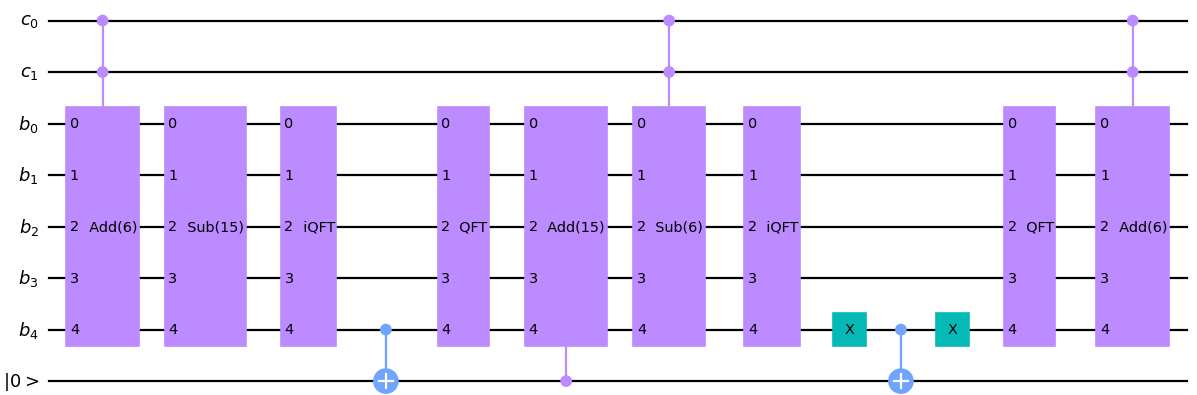
\includegraphics[width=\columnwidth]{modulareAddition.png}
  \centering
  \end{figure}

Abbildung~\ref{fig:ModularAddition} zeigt die Implementierung eines Gatters für die modulare Addition 
mit \(a = 6\) und \(N = 15\) in Qiskit.
Der zugehörige Code, der ein Gatter wie in Abbildung~\ref{fig:ModularAddition} generiert, 
ist in der Funktion \texttt{Modular\_Adder\_Gate}~\ref{code:ModularAddition} enthalten.

Die Funktion \texttt{Modular\_Adder\_Gate} erwartet den Summand \(a\) und die Zahl \(N\) als Parameter, 
jeweils in der Form einer Liste, 
welche die Zahl in Binärdarstellung beschreibt.
Dabei repräsentiert der erste Index beider Listen das Least-Significant-Bit.
Wenn \(N\) der Größenordnung \(2^n\) entspricht, 
müssen die Listen jeweils von der Länge \(n+1\) sein wobei das Most-Significant-Bit immer der \(0\) entspricht.

Die Funktion definiert drei Wertebereiche, die die Positionen der Qubits beschreiben.
\textit{c\_qbits} definiert die Position der beiden Kontroll-Qubits, 
\textit{b\_qbits} die Qubits, welche den Summanden \(b\) 
in der Fourier-Basis enthalten 
und \textit{cond\_qbit} repräsentiert die Position des Bedingungs-Qubit.
Dadurch das \textit{b\_qbits} genau so groß definiert wird, 
wie die Liste des Summand \(a\) lang ist, wird sichergestellt, 
dass das \textit{b\_qbits} Register ein extra Qubit für das Borrow-Bit enthält.
In Zeile 5 der Funktion, wird ein Quantenschaltkreis definiert, 
der aus so viele Qubits besteht, wie es insgesamt an Positionen in 
\textit{c\_qbits}, \textit{b\_qbits} und \textit{cond\_qbit} gibt.

In den Zeilen 6 bis 18 werden alle benötigten Gatter, 
in der selben Reihenfolge wie in Abbildung~\ref{fig:modulare_addition_paper} angewendet.
Zum hinzufügen eines eigens programmierten Gatters, 
also für die Quanten-Addition, Quanten-Subtraktion und die Quanten-Fourier-Transformation,
wird die Qiskit Methode \texttt{append} genutzt.

Abschließend wird der Quantenschaltkreis in Zeile 19 in ein Gatter umgewandelt.

\begin{figure}[H]
  \caption{Modulare Addition in Qiskit}
  \label{code:ModularAddition}
\begin{minted}[linenos,fontsize=\footnotesize]{python}    
def Modular_Adder_Gate(a_bin: list[int],N_bin: list[int]) -> qiskit.circuit.gate:
  c_qbits = [0,1]
  b_qbits = list(range(2, len(a_bin)+2))
  cond_qbit = len(a_bin)+2
  m_a_g = qiskit.QuantumCircuit(2 + len(a_bin) + 1) 
  m_a_g.append(A_Gate(a_bin).control(2), c_qbits + b_qbits)
  m_a_g.append(S_Gate(N_bin),b_qbits)
  m_a_g.append(QFT_Gate(len(a_bin),inverse = True, MSB_first = False), b_qbits)
  m_a_g.cnot(b_qbits[-1],cond_qbit)
  m_a_g.append(QFT_Gate(len(a_bin),inverse = False, MSB_first = False), b_qbits)
  m_a_g.append(A_Gate(N_bin).control(1), [cond_qbit] + b_qbits)
  m_a_g.append(S_Gate(a_bin).control(2), c_qbits + b_qbits)
  m_a_g.append(QFT_Gate(len(a_bin),inverse = True, MSB_first = False), b_qbits)
  m_a_g.x(b_qbits[-1])
  m_a_g.cnot(b_qbits[-1],cond_qbit)
  m_a_g.x(b_qbits[-1])
  m_a_g.append(QFT_Gate(len(a_bin),inverse = False, MSB_first = False), b_qbits)
  m_a_g.append(A_Gate(a_bin).control(2), c_qbits + b_qbits)
  m_a_g = m_a_g.to_gate()
  m_a_g.name = "Add " + str(binToDez(a_bin)) + " Mod " + str(binToDez(N_bin))
  return m_a_g
  \end{minted}
\end{figure}

\subsubsection{Kontrollierte Multiplikation}
Als nächstes wird ein Gatter konstruiert, welches auf vier Quantenregister \(\ket{c}_1\ket{x}_{n}\ket{b}_{n+1}\ket{0}_1\)
eine Transformation nach \(\ket{c}_1\ket{x}_{n}\ket{b + (ax)\mod N}_{n+1}\ket{0}_1\) durchführt.
Das Gatter umfasst ein Kontroll-Qubit \(\ket{c}_1\), 
ein Quantenregister \(\ket{x}_{n}\) mit dem Faktor \(x\),
das Zielregister \(\ket{b}_{n+1}\) mit initialem Wert \(b\) und 
ein Hilfsqubit \(\ket{0}_1\) welches als Bedingungs-Qubit dient.

Die Spezifikation dieses Gatters besteht darin, 
auf den Registerinhalt des Zielregisters \(\ket{b}_{n+1}\) mit initialen Wert \(b\) , 
das Produkt der Faktoren \(x\) und \(a\) modulare aufzuaddieren.

Dabei handelt es sich bei dem Faktor \(a\) um eine vorab bekannte Zahl die während der Berechnung nicht variiert.
Anders sieht dies bei \(x\) aus, da es sich bei dieser Zahl um den Registerinhalt von \(\ket{x}_{n}\) handelt.
Das Gatter berechnet also das Produkt einer klassischen Zahl \(a\) und dem Inhalt eines Quantenregisters \(x\).
Das Register \(\ket{x}_{n}\) umfasst mehrere Qubits die \(x\) im Binärsystem beschreiben, 
also zum Beispiel in Binärschreibweise für drei Qubits \(\ket{x}_{3} = 2^0x_0+2^1x_1+2^2x_2\).
Das Produkt kann dementsprechend umgeformt werden: 
\[(x\cdot a)  = (2^0x_0\cdot a+2^1x_1\cdot a+2^2x_2\cdot a) \]
Beziehungsweise bezogen auf die Transformation des \(\ket{b}_{n+1}\) Registers:
\[\ket{b + (x\cdot a) \mod N}_{4} = \ket{b + (2^0x_0\cdot a+2^1x_1\cdot a+2^2x_2\cdot a) \mod N}_{4}\]
Bedeutet, dass die Transformation realisiert werden kann, 
indem die einzelnen Produkte \(2^ix_i\cdot a\) einzeln auf \(\ket{b}_{n+1}\) addiert werden.
Um große Zwischenergebnisse zu vermeiden, die gegebenenfalls für einen Overflow im \(\ket{b}_{n+1}\) Register sorgen, 
kann man die Berechnung weiter umformen~\cite{beauregard2003circuit}:
\[= \ket{(((b + 2^0x_0\cdot a)\mod N+2^1x_1\cdot a)\mod N+2^2x_2\cdot a) \mod N}_{4}\]
Dies wird als Quantenschaltkreis realisiert, 
indem eine Gatter zur modularen Addition verwendet wird, 
um \((b + 2^ix_i\cdot a)\mod N\) zu berechnet.
Dafür wird das modulare Addition Gatter mit dem Summanden beziehungsweise Parameter \(2^i\cdot a\) versehen 
und für die Abhängigkeit von \(x_i\) durch das Qubit \(\ket{x_i}_1\) kontrolliert.
Für die gesamte Summe muss jedes Qubit des \(\ket{x}_{n}\) Registers ein Gatter zur modularen Addition kontrollieren, 
welche auf das Register \(\ket{b}_{n+1}\) wirken.
Jedes Gatter zur modularen Addition bekommt die zugehörigen Potenz von \(2^i\) zugewiesen, 
die auch der Wertigkeit des zugehörigen Kontroll-Qubits \(\ket{x_i}_1\) entspricht.
Also wirken alle Gatter zur modularen Addition nacheinander auf das \(\ket{b}_{n+1}\) Register und 
Transformieren dies so sukzessiv nach \(\ket{b + (x\cdot a) \mod N}_{n+1}\).

Die verwendeten Gatter zur modularen Addition führen alle Berechnungen in der Fourier-Basis durch.
Deswegen muss sich das \(\ket{b}_{n+1}\) Register auch in der Fourier-Basis befinden.
Das Gatter für die kontrollierte Multiplikation wirkt dazu als erste Operation eine Quanten-Fourier-Transformation auf 
das Zielregister \(\ket{b}_{n+1}\) und als letzte Operation die inverse Quanten-Fourier-Transformation.

Zusätzlich verfügt das Gatter zur kontrollierten Multiplikation noch über das Kontroll-Qubit \(\ket{c}_1\).
Dieses Kontroll-Qubit kontrolliert alle der verwendeten modularen Addition Gatter.
Das Kontroll-Qubit \(\ket{c}_1\) findet beim nächsten Gatter Gebrauch.

Alles zusammen führt zu einem Quantenschaltkreis wie in Abbildung~\ref{fig:cmult}.
\begin{figure} [H]
  \caption{Kontrollierte Multiplikation nach Beauregard~\cite{beauregard2003circuit}}
  \label{fig:cmult}
  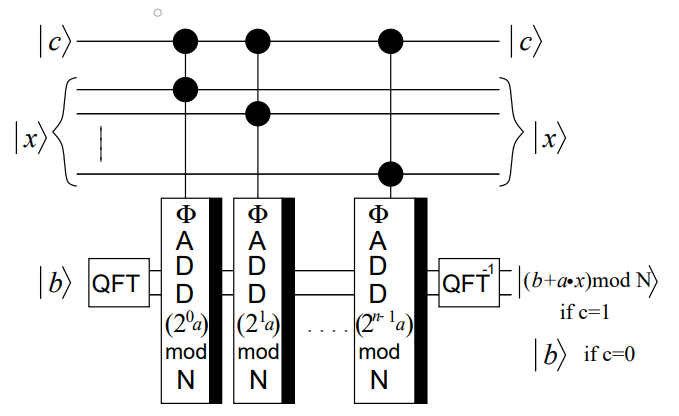
\includegraphics[scale = 0.6]{cmult.png}
  \centering
  \end{figure}



\vspace{1em}

Der Code der einen Quantenschaltkreis als Gatter nach dem Konzept in Abbildung~\ref{fig:cmult} generiert, 
wird in der Funktion \texttt{cmult\_gate}~\ref{code:ModularMultiplication} definiert.
Die Funktion erwartet sowohl \(a\) als auch \(N\) als Parameter, 
jeweils in der Form einer Liste, welche die Zahl in Binärdarstellung beschreibt.
Dabei repräsentiert der erste Index beider Listen das Least-Significant-Bit.
Damit die unterliegenden modularen Addition Gatter für die korrekte Anzahl an Qubits gebildet werden, 
müssen die Listen jeweils von der Länge n + 1 sein, wenn \(N\) der Größenordnung \(2^n\) entspricht.
Das Most-Significant-Bit ist dementsprechend für beide Listen \(0\).
Des Weiteren erwartet die Funktion den Parameter \textit{x\_bits\_amount}, welcher angibt, 
wie viele Qubits das Register \(\ket{x}_n\) umfasst 
und somit also \(n\) entspricht. 

Um die Position der Qubits zu beschreiben, 
werden in der Funktion vier Wertebereiche definiert.
\textit{c\_qbit} liegt an der ersten Stelle des kontrollierten Multiplikation Gatters und 
ist für das Kontroll-Qubit \(\ket{c}_1\) vorhergesehen.
Die darauffolgenden Qubits umfassen das \(\ket{x}_n\) Register und bestehen aus insgesamt \(n\) Qubits, 
deren Position in \textit{c\_qbit} definiert ist.
Die Position des \(\ket{b}_{n+1}\) Registers wird in \textit{b\_qbits} beschrieben.
Aufgrund der unterliegenden Gatter umfasst das \(\ket{b}_{n+1}\) Register ein extra Qubit, 
welches als Borrow-Bit dient.
Die Position des letzten Qubit \(\ket{0}_1\) wird mit \textit{cond\_qbit} definiert.
Dieses Qubit ist das Bedingungs-Qubit für die unterliegenden modularen Addition Gatter.

Im Code~\ref{code:ModularMultiplication} wird in Zeile 9 die Quanten-Fourier-Transformation auf 
das \(\ket{b}_{n+1}\) Register anwendet.
In Zeile 10 bis 13 folgen die Gatter zur modularen Addition.
Da \((b + a \cdot x) \mod N\) äquivalent ist zu \((b + (a \cdot x)\mod N) \mod N\)~\cite{koepf_modular_2021}, 
wird einem Gatter der modularen Addition nicht der Parameter \(2^i\cdot a\) übergeben, 
sondern \((2^i\cdot a)\mod N\).
Andernfalls wäre es nötig, 
zusätzliche Qubits zu verwendet, 
damit \(2^i\cdot a\) gespeichert werden kann.
Wie man in Zeile 13 sieht, teilen sich alle modularen Additions Gatter das selbe Bedingungs-Qubit \(\ket{0}_1\), 
welches sich auf der Position von \textit{cond\_qbit} befindet.
Genau aus diesem Grund, wird bei dem Gatter zur modularen Addition des Bedingungs-Qubit zurückgesetzt.
Abschließend wird noch die inverse Quanten-Fourier-Transformation auf das \(\ket{b}_{n+1}\) Register anwendet und 
von einem Quantenschaltkreis in ein Quantengatter umgeformt.

\begin{figure}[H]
  \caption{Kontrollierte Multiplikation in Qiskit}
  \label{code:ModularMultiplication}
\begin{minted}[linenos,fontsize=\footnotesize]{python}  
def cmult_gate(x_bits_amount: int,a_bin: list[int],N_bin: list[int]) -> qiskit.circuit.gate:  
  a_dez = binToDez(a_bin)
  N_dez = binToDez(N_bin)
  c_qbit = [0]
  x_qbits =  list(range(1, x_bits_amount + 1))
  b_qbits = list(range(1+x_bits_amount, 1 + x_bits_amount + len(a_bin)))
  cond_qbit = [1 + x_bits_amount + len(a_bin)]
  cmult_gate = qiskit.QuantumCircuit(1 + x_bits_amount + len(a_bin) + 1)
  cmult_gate.append(QFT_Gate(len(b_qbits),inverse = False, MSB_first = False), b_qbits)
  for i in range(0, len(x_qbits)):
      a_i = ((2**(i)) *  a_dez) % N_dez
      a_i_bin = dezToBin(a_i, len(a_bin))
      cmult_gate.append(modular_adder_gate(a_i_bin, N_bin),c_qbit+[x_qbits[i]]+b_qbits+cond_qbit)
  cmult_gate.append(QFT_Gate(len(b_qbits),inverse = True, MSB_first = False), b_qbits)
  cmult_gate = cmult_gate.to_gate()
  cmult_gate.name = "cmult " + str(a_dez) + " Mod " + str(N_dez)
  return cmult_gate
  \end{minted}
\end{figure}

In Qiskit wird der durch den Code gebildete Quantenschaltkreis wie in Abbildung~\ref{fig:cmult_qiskit} in Qiskit dargestellt.
Die Visualisierung der Kontroll-Abzweigungen ist anders als in den vorherigen Abbildungen dargestellt.
Dies liegt daran, dass die Kontroll-Qubits bereits in den unterliegenden Gattern, 
also der modularen Addition, 
definiert wurden.
Es ist möglich, die Kontroll-Qubits bei der Definition der modularen Adder Gatter auszulassen und 
stattdessen erst bei der Anwendung im kontrollierten Multiplikation Gatter anzuwenden, 
indem die Qiskit Funktion \textit{control} verwendet wird.
Dadurch wird der Kontrolleffekt auf das gesamte Gatter zur modularen Addition angewendet, 
wodurch man einen ineffizientere Quantenschaltkreis erhält, 
wie bereits im Abschnitt~\ref{sub:modulareAddition} zur modularen Addition erwähnt.

Es ist zu beachten, dass die Gatter zur modularen Addition in Abbildung~\ref{fig:cmult_qiskit} zwar über 
alle Qubits des \(\ket{x}_n\) Registers verlaufen, 
jedoch ausschließlich durch das Qubit kontrolliert werden, 
bei dem das modularen Additions Gatter den Index 1 verzeichnet.
Die Abbildung repräsentiert den Quantenschaltkreis für \(a = 11;~N = 15\).

\begin{figure} [H]
  \caption{Schaltkreis der kontrollierten Multiplikation in Qiskit}
  \label{fig:cmult_qiskit}
  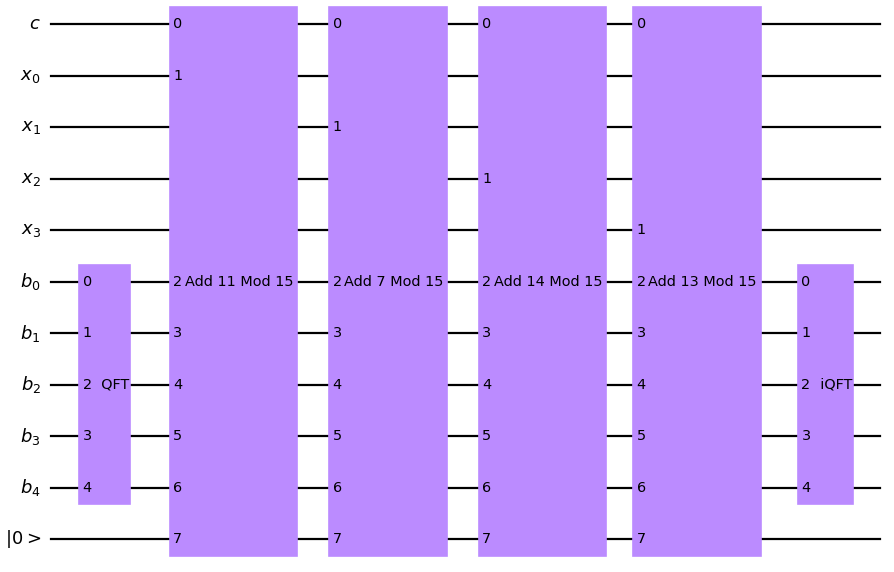
\includegraphics[scale = 0.5]{cmult_qiskit.PNG}
  \centering
  \end{figure}

Insgesamt wirkt das Gatter auf \(2n+3\) Qubits.
Diese setzen sich aus dem Kontroll-Qubit \(\ket{c}_1\), den \(n\) Qubits von \(\ket{x}_n\), 
den \(n+1\) Qubits von \(\ket{b}_{n+1}\) und dem Bedingungs-Qubit \(\ket{0}_1\)zusammen.

Damit die Inverse des kontrollierten Multiplikation Gatters eine Eindeutige Benennung hat, 
wird dafür eine zusätzliche Funktion \texttt{inv\_cmult\_gate} definiert.
\begin{figure}[H]
  \caption{Inverse kontrollierte Multiplikation in Qiskit}
  \label{code:InverseModularMultiplication}
\begin{minted}[linenos,fontsize=\footnotesize]{python}  
def inv_cmult_gate(x_bits_amount: int,a_bin: list[int],N_bin: list[int]) -> qiskit.circuit.gate:  
  inv_cmult_gate = cmult_gate(x_bits_amount,a_bin,N_bin).inverse()
  inv_cmult_gate.name = "inv cmult " + str(binToDez(a_bin)) + " Mod " + str(binToDez(N_bin))
  return inv_cmult_gate
  \end{minted}
\end{figure}

\subsubsection{Vollstände Transformation}

Das letzte zu konstruierende Gatter realisiert die benötigte Transformation \(U\ket{y} = \ket{ay \mod N}\) und 
wird im weiteren als \(U_a\)-Gatter bezeichnet.
Mit dem \(U_a\)-Gatter wird die Quanten-Phase-Estimation, 
wie in Abbildung~\ref{fig:shor_n_qubit}, für den Shor-Algorithmus gebildet.
Dafür nimmt das \(U_a\)-Gatter die Quantenregister \(\ket{c}_1\ket{x}_{n}\ket{0}_{n+1}\ket{0}_1\) entgegen und 
führt eine Transformation nach \(\ket{c}_1\ket{(a \cdot x) \mod N}_{n}\ket{0}_{n+1}\ket{0}_1\) durch.

Um ein \(U_a\)-Gatter zu realisieren, benötigt man im Grunde lediglich zwei Gatter zur kontrollierten Multiplikation und 
kontrollierte Swap-Gatter. 

Im folgenden wird die Auswirkung der einzelnen Bestandteile des \(U_a\)-Gatter erklärt.
Dabei werden von den Quantenregistern \(\ket{c}_1\ket{x}_{n}\ket{0}_{n+1}\ket{0}_1\) nur die beiden 
Quantenregister \(\ket{x}_{n}\ket{0}_{n+1}\) beachtet.
Sowohl \(\ket{c}_1\) also auch \(\ket{0}_1\) verzeichnen während der Transformation keine Veränderung, 
welche für das Verständnis des \(U_a\)-Gatters relevant ist.
Der Ablauf des \(U_a\)-Gatter ist der folgende~\cite{beauregard2003circuit}:
Initial befindet sich die beiden Quantenregistern in dem Zustand \(\ket{x}_{n}\ket{0}_{n+1}\), 
anschließend wird ein Gatter zur kontrollierten Multiplikation mit \(a\) ausgeführt, 
welches den Zustand zu \(\ket{x}_{n}\ket{(ax)\mod N}_{n+1}\) transformiert.
Darauf folgen kontrollierte Swap-Gatter die beide Zustände zu \(\ket{(ax)\mod N}_{n}\ket{x}_{n+1}\) vertauschen.
Dabei ist zu beachten, 
dass das zweite Quantenregister aus \(n+1\) Gattern besteht, 
also ein Qubit mehr besitzt, als das erste Quantenregister.
Da das Most-Significant-Bit des zweiten Quantenregisters, zu dem Zeitpunkt, garantiert dem Zustand \(\ket{0}\) entspricht, 
kann dieses Vernachlässigt werden und wird keiner Swap-Operation unterzogen.
Nach dem Swap wird ein inverses Gatter zur kontrollierten Multiplikation angewendet.
Des Weiteren wird dem inverses Gatter zur kontrollierten Multiplikation statt dem Element \(a\), 
das inverse von \(a\) sein multiplikatives Inverses in den Einheiten des Restklassenrings \(N\) übergeben, 
also \(a^{-1} \mod N\).
Als Folge davon, verändert sich der Zustand der Quantenregister von \(\ket{(ax)\mod N}_{n}\ket{x}_{n+1}\) 
zu \(\ket{(ax)\mod N}_{n}\ket{(x-a^{-1}ax)\mod N}_{n+1}\).
Der Ausdruck \((a^{-1}a)\mod N\) entspricht dem neutralen Element 1, 
weswegen der Zustand der Quantenregister zu \(\ket{(ax)\mod N}_{n}\ket{0}_{n+1}\) vereinfacht werden kann.

Beachtet man also den ersten und letzten Zustand der beiden Quantenregister, 
so bewirkt das \(U\)-Gatter also eine Transformation von \(\ket{x}_{n}\ket{0}_{n+1}\) zu \(\ket{(ax)\mod N}_{n}\ket{0}_{n+1}\).
Das Konzept des Aufbaus des Quantenschaltkreises ist in Abbildung~\ref{fig:u_gatter} dargestellt.
\begin{figure} [H]
  \caption{\(U_a\)-Gatter~\cite{beauregard2003circuit}}
  \label{fig:u_gatter}
  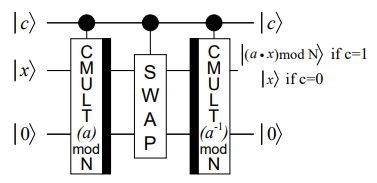
\includegraphics[scale = 0.8]{u_gatter.png}
  \centering
  \end{figure}

Die Funktion \texttt{U\_gate}~\ref{code:UGatter} enthält den Code um ein \(U_a\)-Gatter zu generieren.
Dazu benötigt die Funktion die selben Parameter wie die Funktion \texttt{cmult\_gate}, 
also \textit{a\_bin} und \textit{N\_bin}, welche jeweils \(a\) und \(N\) binär im Listenformat beschreibt und 
\textit{x\_bits\_amount}, die im Grunde \(n\) repräsentiert.

Im Code~\ref{code:UGatter} werden insgesamt fünf Wertebereiche definiert.
Das Kontroll-Qubit \(\ket{c}_1\) befindet sich auf der Position \textit{c\_qbit}.
Das \(\ket{x}_{n}\) Quantenregister wird durch \textit{x\_qbits} beschrieben, 
gefolgt von \textit{b\_qbits} für die Qubits von \(\ket{0}_{n+1}\).
Das Bedingungs-Qubit wird auf der letzten Position des Gatters platziert, die in \textit{cond\_qbit} festgelegt ist.
Des Weiteren wird noch \textit{full\_range} verwendet,
in welcher alle der vier vorherigen Quantenregister umfasst sind.

Wie im Code in Zeile 7 zu sehen ist, wird zuerst ein Gatter zur kontrollierten Multiplikation eingesetzt.
Dazu bekommt die Funktion \texttt{cmult\_gate} die Parameter \textit{a\_bin}, \textit{N\_bin} und \textit{x\_bits\_amount} übergeben.
Das Gatter zur kontrollierten Multiplikation wird über den Bereich \textit{full\_range} angewendet, 
somit umfasst das \(U_a\)-Gatter auch \(2n+3\) Qubits.
In Zeile 9 und 10 werden die kontrollierten Swap-Gatter eingesetzt.
Wie man in Zeile 10 erkennt, bezieht sich die Wirkung eines Swap-Gatters auf den selben index von \textit{x\_qbits} und \textit{b\_qbits}.
Somit werden die Qubits beider Quantenregister vertauscht, die die identische Wertigkeit besitzen.
In Zeile 11 wird \(a^{-1}\mod N\) mit dem erweiterte euklidische Algorithmus Berechnet.
Anschließend wird das Berechnete \(a^{-1}\mod N\) als Parameter an ein inverses kontrolliertes Multiplikation Gatter übergeben.
Abschließend wird der Quantenschaltkreis zu einem Gatter umgeformt und passend benannt.

\begin{figure}[H]
  \caption{\(U\)-Gatter in Qiskit}
  \label{code:UGatter}
\begin{minted}[linenos,fontsize=\footnotesize]{python}  
def U_gate(x_bits_amount: int,a_bin: list[int],N_bin: list[int]) -> qiskit.circuit.gate:  
  c_qbit = [0]
  x_qbits =  list(range(1, x_bits_amount + 1))
  b_qbits = list(range(1+x_bits_amount, 1 + x_bits_amount + len(a_bin)))
  cond_qbit = [1 + x_bits_amount + len(a_bin)]
  full_range = c_qbit + x_qbits + b_qbits + cond_qbit
  U_a_gate = qiskit.QuantumCircuit(len(full_range))
  U_a_gate.append(cmult_gate(x_bits_amount,a_bin ,N_bin), full_range)
  for i in (range(x_bits_amount)):
      U_a_gate.cswap(c_qbit,x_qbits[i],b_qbits[i])
  a_inv_bin = dezToBin(gcd(binToDez(a_bin),binToDez(N_bin)),len(a_bin))
  U_a_gate.append(inv_cmult_gate(x_bits_amount,a_inv_bin ,N_bin), full_range)
  U_a_gate = U_a_gate.to_gate()
  U_a_gate.name = "  U_" + str(binToDez(a_bin))
  return U_a_gate
  \end{minted}
\end{figure}

Der Quantenschaltkreis der durch den Code~\ref{code:UGatter} gebildet wird, 
wird in Qiskit wie in Abbildung dargestellt. 
Die Abbildung~\ref{fig:u_gatter_qiskit} zeigt ein Beispiel für \(a=7\) und \(N=15\).

\begin{figure} [H]
  \caption{\(U_a\)-Gatter in Qiskit}
  \label{fig:u_gatter_qiskit}
  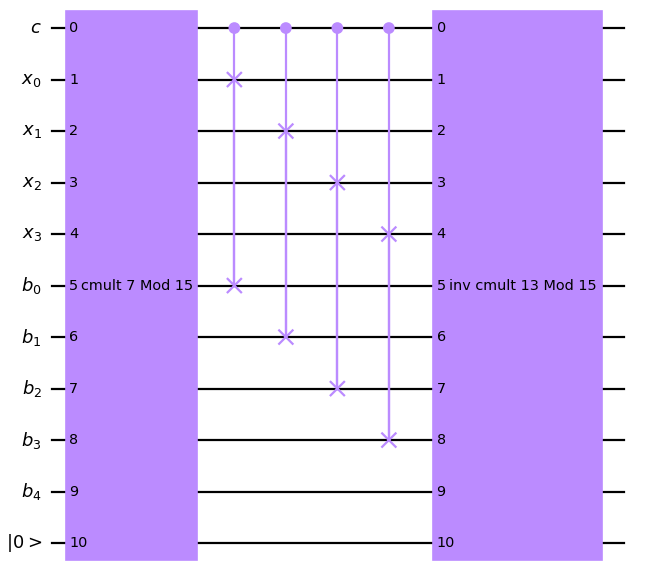
\includegraphics[scale = 0.5]{u_gatter_qiskit.PNG}
  \centering
  \end{figure}

\subsubsection{QPE für Shor}
Das \(U_a\)-Gatter führt die benötigte unitäre Transformation von \(U\ket{y} = \ket{ay \mod N}\) aus.
Der letzte Schritt, um den Quantenschaltkreis des Quantenalgorithmus zu bilden, 
der in der Lage, ist die Periode zu bestimmen, 
besteht darin, 
die Quanten-Phase-Estimation wie in Abbildung~\ref{fig:shor_n_qubit} mit den \(U_a\)-Gatter nachzubauen.

In Abbildung~\ref{fig:shor_n_qubit} werden unter anderem \({U_a}^{2^x}\)-Gatter eingesetzt.
Diese können realisiert werden, 
indem ein \({U_a}\)-Gatter insgesamt \(2^x\) mal hintereinander geschaltet wird oder 
indem anstelle von \(a\) den Parameter \(a^{2^x}\) an ein einzelnes \(U_a\)-Gatter übergibt.
Die zweite Variante ist möglich wegen~\cite{beauregard2003circuit}:
\[(a^nx)\mod N = \underbrace{(a...(((a(ax)\mod N)\mod N)...)\mod N)}_{\text{\(n\) mal}}\]

Bei der Wahl zwischen den beiden Varianten ist das entscheidende Kriterium bei der Ressourceneffizienz. 
Die zweite Variante schneidet dabei deutlich besser ab, da sie lediglich \(2n\) \(U_a\)-Gatter benötigt, 
im Gegensatz zur ersten Variante, die \(2^n-1\) \(U_a\)-Gatter erfordert.

Ein weiterer wichtiger Aspekt für den Aufbau der Quantenschaltung betrifft die Anzahl der benötigten Kontroll-Qubits.
Beauregard erklärt in seinem Paper~\cite{beauregard2003circuit} nicht, 
warum er eine Konstruktion mit insgesamt \(2n\) Kontroll-Qubits beziehungsweise \({U_a}^{2^x}\)-Gatter wählt.
Es gibt Quellen, die mehr als \(2n\) \({U_a}^{2^x}\)-Gatter verwendeten~\cite{nielsen_chuang_2010}.
Nach dem Paper von Peter Shor~\cite{Shor_1997} sind jedoch \(2n\) \({U_a}^{2^x}\)-Gatter ausreichen,
wie auch im Abschnitt~\ref{Funktionsweise:klassisch} erläutert wird.
Deswegen verwendet die hier implementierte Variante \(2n\) Kontroll-Qubits.

\vspace{1em}

Der Code für einen Quantenschaltkreis wie in Abbildung~\ref{fig:shor_n_qubit} ist in der Funktion 
\texttt{Shor}~\ref{code:Periodenbestimmung} enthalten.
Die Funktion erwartet die beiden Zahlen \(a\) und \(N\) als Parameter.
Des Weiteren kann der Funktion über den Parameter \textit{number\_shots} mitgeteilt werden, 
mit wie vielen Durchläufen der Quantenalgorithmus ausgeführt werden soll.
Jeder Durchlauf gewährt ein weiteres Messergebnis.
Der Parameter \textit{backend} ist dazu da, 
um Festzulegen auf welchem System der Quantenalgorithmus ausgeführt werden soll.
Standardmäßig wird der Simulator von Qiskit genommen, 
falls Zugang zu einem Quantensystem von IBM besteht, 
würde man hier die Bezeichnung des entsprechenden Quantum-Backend verwenden.
Die Funktion \texttt{Shor} definiert die beiden Wertebereiche \textit{c\_qbits} und 
\textit{ev\_qbits} um die Positionen der beiden Quantenregister zu beschreiben.
Der Wertebereich \textit{c\_qbits} enthält die insgesamt \(2n\) Positionen der Kontroll-Qubits.
Der Eigenvektor wird in den Qubits gespeichert, 
deren Position in \textit{ev\_qbits} definiert ist.
Der Quantenschaltkreis wird in der 5 Zeile definiert und umfasst \(4n+2\) Qubits und 
\(2n\) klassische Bits, welche zum Messen verwendet werden.
In Zeile 6 und 7 wird auf jedes Kontroll-Qubit mit ein Hadamard-Gatter angewendet.
In Zeile 8 wird der Eigenvektor gebildet. 
Da dieser dem Zustand \(\ket{1}\) entspricht,
genügt es, wenn das Least-Significant-Qubit mit einem X-Gatter versehen wird.
Die Zeile 9 und 10 wendet das Zugehörige \({U_a}^{2^x}\)-Gatter mit dem passenden \(x\) auf das Register mit dem Eigenvektor an.
Die Funktion \texttt{mod\_exp} berechnet \((a^{2^x})\mod N\).
In Zeile 11 wird die inverse Quanten-Fourier-Transformation auf die Kontroll-Qubits angewendet.
Da die Funktion \texttt{Shor} Messungen durchführen soll, 
wird in Zeile 12 definiert, welche Qubits gemessen werden. 
Anschließend werden in Zeile 13-14 \textit{number\_shots} viele Messungen durchgeführt und 
das Ergebnis als Rückgabewert der Funktion zurückgeben.

Wie bei der Definition des Quantenschaltkreis in Zeil 5 erkennbar, 
benötigt der Quantenschaltkreis \(4n+2\) Qubits anstatt \(2n+3\).
Die Reduktion der benötigten Qubits wird in der Sektion~\ref{Optimierung} thematisiert. 

\begin{figure}[H]
  \caption{Periodenbestimmung in Qiskit}
  \label{code:Periodenbestimmung}
\begin{minted}[linenos,fontsize=\footnotesize]{python}  
def Shor(a: int, N: int,number_shots: int = 1000, backend: str = "aer_simulator"):
  n = N.bit_length()
  c_qbits = range(2*n)
  ev_qbits = list(range(len(c_qbits),4*n+2))
  qc = qiskit.QuantumCircuit(4*n+2,len(c_qbits)) 
  for c_bit in c_qbits:
    qc.h(c_bit)
  qc.x(ev_qbits[0])
  for c_bit in c_qbits:
    qc.append(U_gate(n,dezToBin(mod_exp(a,2**c_bit,N),n+1),dezToBin(N,n+1)),[c_bit]+ev_qbits)
  qc.append(QFT_Gate(len(c_qbits),inverse = True, MSB_first = False,swaps = True), c_qbits)
  qc.measure(c_qbits,c_qbits)
  simulator = qiskit.Aer.get_backend(backend)
  sim_result = qiskit.execute(qc, backend=simulator, shots=number_shots).result()
  return sim_result.get_counts(qc)
  \end{minted}
\end{figure}

In Abbildung~\ref{fig:shor_qiskit} ist der Quantenschaltkreis zu sehen, 
welcher durch die Funktion \texttt{Shor} mit \(a=7;~N=15\) generiert wird.
Bei \(N=15\) tritt der Effekt auf, das für \(x>1\) die Rechnung \((a^{2^x})\mod N = 1\) ergibt, 
weswegen auch die \({U_a}^{2^x}\)-Gatter zu \(U_1\) werden.

\begin{figure} [H]
  \caption{Quantenalgorithmus von Shor in Qiskit}
  \label{fig:shor_qiskit}
  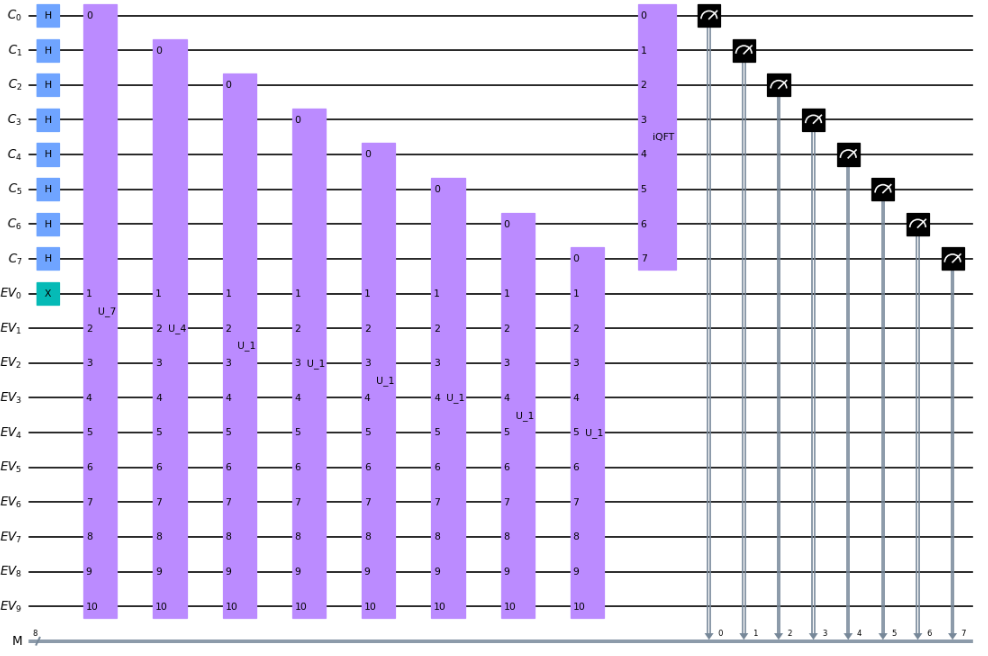
\includegraphics[scale = 0.6]{shor_qiskit.PNG}
  \centering
  \end{figure}

\subsection{Faktorisierungsalgorithmus}
Der Faktorisierungsalgorithmus kombiniert die Quanten-Phase-Estimation zur Periodenberechnung mit  
der klassischen Nachberechnung. 
Der Hauptfokus der Implementierung liegt darauf, 
die Schwächen der Messergebnisse der Quanten-Phase-Estimation mithilfe klassischer Methoden zu kompensieren.
Es ist zu erwarten, 
dass die Ausführung von Quantenberechnungen auch mit zukünftig fortschrittlichen Quantencomputern kostenintensiv sein wird~\cite{Shor_1997}.
Daher wäre es ineffizient, 
die die Quanten-Phase-Estimation so oft zu wiederholen, 
bis ein Ergebnis erzielt wird, das die Periode direkt offenbart.
Stattdessen ist es ressourcensparender, ein erhaltenes Messergebnis 
unter Berücksichtigung der drei möglichen Szenarien 
die in Abschnitt~\ref{Funktionsweise:klassisch} erklärt werden,
mit klassischen Methoden aufzubereiten. 
Als Resultat können so weitere Durchläufe der Quanten-Phase-Estimation eingespart und 
durch klassische Rechenleistung ersetzt werden.

\vspace{1em}

Die Grafik~\ref{fig:shor_measure} repräsentiert insgesamt 512 Messungen für \(a=19;~N=119\), 
mit einer Genauigkeit \(k\) von \(2\text{ld}(119) \approx 14 \) und soll die Besonderheiten, 
welche bei Messergebnissen auftreten können, hervorheben.
Zur Verdeutlichung sind die Messergebnisse in Abbildung~\ref{fig:shor_measure} in vier Kategorien eingeteilt.
Die Kriterien für die Einteilung in diese Kategorien basieren darauf, 
ob nach der Division durch \(2^k\) und 
der Anwendung des Kettenbruch-Algorithmus mit einem Limit von \(N\), 
die Periode erfolgreich extrahiert werden kann.

Die grünen Ergebnisse offenbaren direkt die gesuchte Periode von \(p = 24\).
Ein Faktorisierungsalgorithmus der solange die Quanten-Phase-Estimation wiederholt, 
bis ein Messergebnis die ungekürzte Periode enthält, 
wird ausschließlich bei den grünen Ergebnissen erfolgreich sein.

Anhand der gelben Ergebnisse kann die gesuchte Periode nicht direkt extrahiert werden.
Dabei ist der Fall eingetreten, dass der Zähler und Nenner des Bruches einen gemeinsamen Teiler hatte, 
wodurch der Bruch gekürzt werden konnte.
Gegebenenfalls kann die Periode mit klassisch ausführbaren Methoden rekonstruiert werden.

Die hellroten Ergebnisse sind zu weit vom Peak entfernt,
weswegen diese die gesuchte Periode weder vollständig noch gekürzt enthalten.
Womöglich kann von diesem Messergebnis die Periode gefunden werden, 
wenn man die benachbarten Zustände überprüft.

Die beiden dunkelroten Zustände sind die beiden Zustände der finale Superposition
\(\ket{2^k \cdot \frac{0}{p}}_k\) und \(\ket{2^k \cdot \frac{p/2}{p}}_k\).
Der Zustand \(\ket{2^k \cdot \frac{0}{p}}_k\) existiert für jede Zahl und erlaubt keine 
Rückschlüsse auf die Periode.
Der andere Zustand \(\ket{2^k \cdot \frac{p/2}{p}}_k\) existiert ausschließlich wenn \(p\) gerade ist.
Auch dieser Zustand gewehrt keine hilfreichen Rückschlüsse auf die Phase, 
da \(\frac{p/2}{p}\) immer zu \(\frac{1}{2}\) gekürzt wird.
Eine notwendige Bedingung um die Faktoren aus \(p\) herleiten zu können, 
ist, das \(p\) gerade ist~\cite*{Shor_1997}, 
dies wird zwar durch die Messung von \(\ket{2^k \cdot \frac{p/2}{p}}_k\) bestätigt, 
jedoch kann aus dieser Information keine hilfreiche Konsequenz gezogen werden.

\begin{figure} [H]
\caption{Beispiel Messung}
\label{fig:shor_measure}
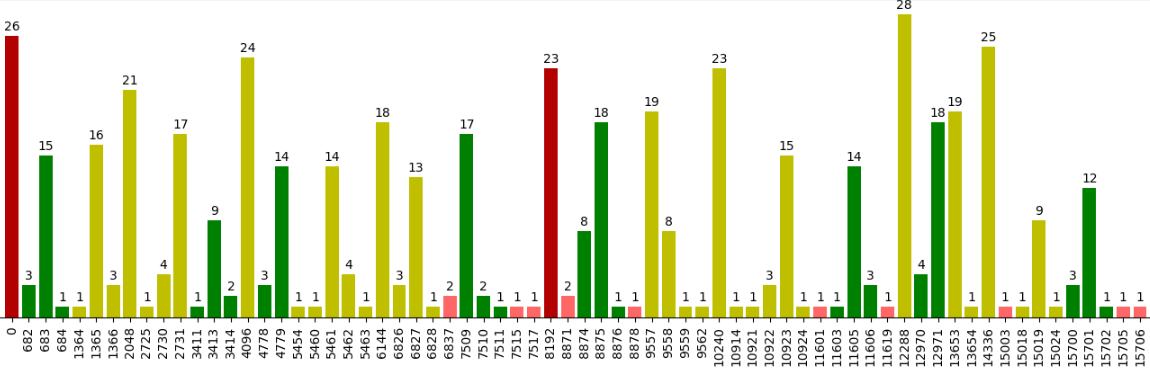
\includegraphics[scale = 0.5]{Messung_beispiel.PNG}
\centering
\end{figure}

\vspace{1em}

Das Flussdiagramm in Abbildung~\ref{fig:Flussdiagramm} beschreibt den 

\begin{figure} [H]
\caption{Flussdiagramm Faktorisierung}
\label{fig:Flussdiagramm}
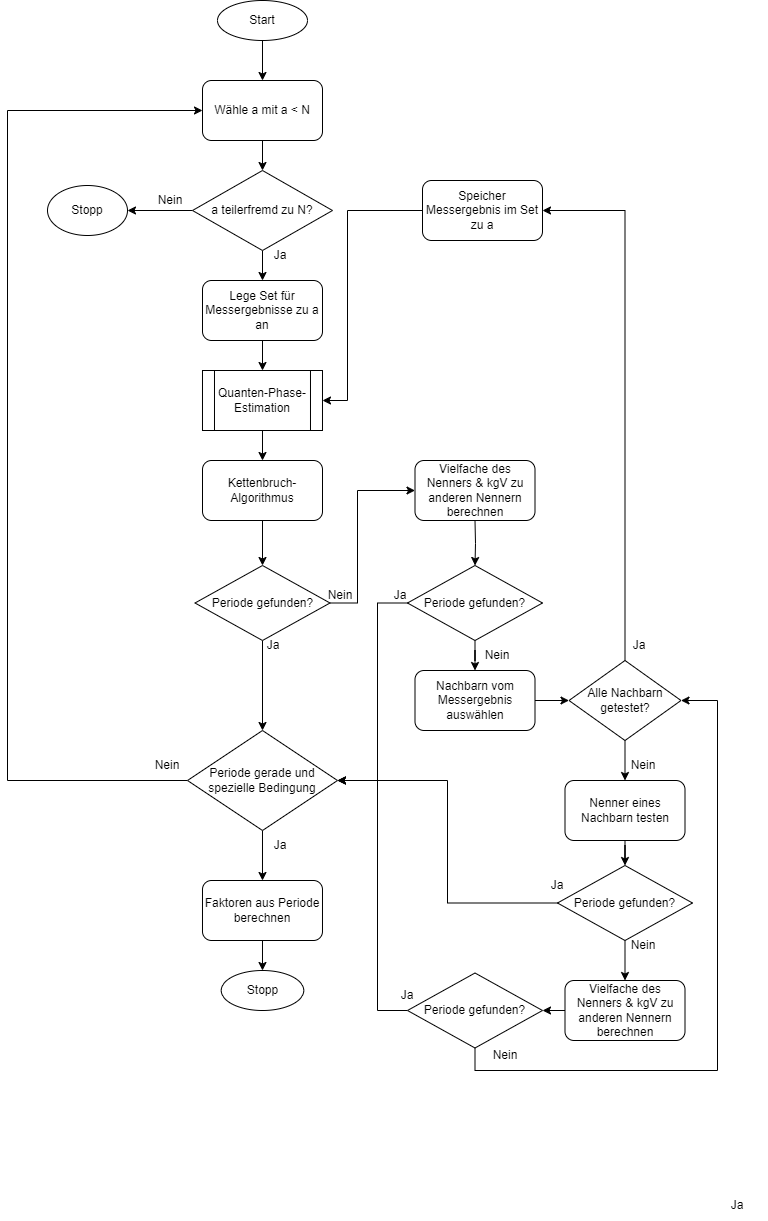
\includegraphics[scale = 0.5]{FlussdiagramFaktorisierung.png}
\centering
\end{figure}

\subsection{Optimierung} \label{Optimierung}


